\usepackage{tikz-cd}
\begin{document}
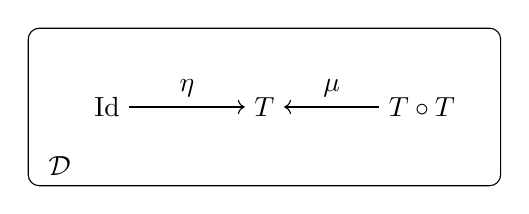
\begin{tikzpicture}
  \draw[rounded corners] (-3,-1) rectangle (3,1);
  \node at (-2.6,-0.75) {$\mathcal{D}$};
  \node (Id) at (-2,0) {$\mathrm{Id}$};
  \node (T) at (0,0) {$T$};
  \node (TT) at (2,0) {$T \circ T$};
  \draw[->] (Id) -- node[above] {$\eta$} (T);
  \draw[->] (TT) -- node[above] {$\mu$} (T);
\end{tikzpicture}
\end{document}
